\section{Simulated AT-TPC events}
The simulated AT-TPC tracks were simulated with the \lstinline{pytpc} package developed at the NSCL\todo{citation}. Using the same parameters as for the $Ar^{46}(p, p)$ experiment a set of $N=4000$ events were generated per class. The events are generated in the same format as the semi-raw experimental data. That is they are represented as peak-only 4-tuples of $e_i = (x_i, y_i, t_i, c_i)$. Each event is then a set of these four-tuples: $\epsilon_j = \{e_i\}$ creating a track in three dimensional space with charge amplitude for each point. To process these events with the algorithms implemented for this thesis we chose to represent these 3D tracks as 2D images with charge represented as pixel images. For the analysis we chose to view the x-y projection of the data \todo{figure of 3D simulated track and 2D representation}

\subsection{Classification of events} 
From the simulated data we have two classes of events; proton and carbon. Our hypothesis is that we can separate these with a linear classifier, additionally we will investigate how many labeled samples we need to achieve good classification. The investigation of the performance will be separated in the sequential and non\-sequential models. The simulated data is very simple and does not necessitate the full hyperparameter search machinery. We begin by considering the non-sequential Autoencoders.

\subsubsection{Convolutional Autoencoder classification results\protect\footnote{The scripts used to produce the results for this section can be found in the repository at: \lstinline{scripts/convae_simulated.py}, \lstinline{notebooks/draw_model.ipynb}, and \lstinline{notebooks/latent_space_simulated.ipynb}}}

The training procedure for classification using a semi-supervised regime as the one we'll apply necessitates the same strict separation of labeled data for the classification step as when considering ordinary classification tasks. To emulate the real-data case we set a subset of the simulated data to be labeled and treat the rest as unlabeled data. We chose this partition to be $15\%$ of each class. We denote this subset and its associated labels as $\gamma_L=(\mathbf{X}_L, \mathbf{y}_L)$, the entire dataset which we will denote as $\mathbf{X}_F$. To clarify please note that $\mathbf{X}_L \subset \mathbf{X}_F$. Furthermore, the tuple $\gamma_L$ has to be split in training and test sets. The test partition is set to be $30\%$ of the samples. The model hyperparameters were heuristically chosen to conform with current best practices, but the simulated data is presents such a simple learning task that good results can be easily obtained. The hyperparameters as chosen are listed in table \ref{tab:param_vals_sim_convae}. We estimate the classification performance over $N=10$ experiments and list the results in table \ref{tab:clf_simulated}. The classifier was a logistic regression model from the \lstinline{scikit-learn} python library trained on the expressions of the image-data.

\begin{table}
\centering
\setlength{\extrarowheight}{15pt}
\hspace*{-0.5in}
\begin{tabular}{|l|l|}
\hline
Hyperparameter & Value \\
\hline \hline
\multicolumn{2}{|l|}{Convolutional parameters: } \\
\hline
Number of layers & 4\\
Kernels & $[5,\, 5,\, 3,\, 3]$\\
Strides & $[2,\, 2,\, 2,\, 2]$\\
Filters & $[8,\, 16,\, 32,\, 64]$ \\ 
\hline
\multicolumn{2}{|l|}{Network parameters: } \\
\hline
Activation & ReLU \\
Latent type & MMD \\
Latent dimension & $3$ \\
$\beta$ & \num{1e-1} \\
\hline
\multicolumn{2}{|l|}{Optimizer parameters: } \\
\hline
$\eta$ &  \num{1e-2} \\
$\beta_1$ & $0.7$ \\
$\beta_2$ & $0.99$ \\
\hline
\end{tabular}
\caption{Hyperparameters chosen for the convolutional autoencoder when training on the simulated data}\label{tab:param_vals_sim_convae}
\end{table}

\begin{table}
\begin{tabular}{l|ccc|ccc}
 & \multicolumn{3}{c}{Proton} & \multicolumn{3}{c}{Carbon} \\
 \hline
 & f1 & recall & precision & f1 & recall & precision\\
 Train & $ \underset{ \num{+- 4.94e-02 } } {\num{ 0.62 } }  $ & $ \underset{ \num{+- 5.51e-02 } } {\num{ 0.62 } }  $ & $ \underset{ \num{+- 4.82e-02 } } {\num{ 0.61 } }  $ & $ \underset{ \num{+- 6.81e-02 } } {\num{ 0.63 } }  $ & $ \underset{ \num{+- 5.78e-02 } } {\num{ 0.63 } }  $ & $ \underset{ \num{+- 4.72e-02 } } {\num{ 0.61 } }  $ \\
  Test & $ \underset{ \num{+- 3.85e-02 } } {\num{ 0.61 } }  $ & $ \underset{ \num{+- 6.00e-02 } } {\num{ 0.63 } }  $ & $ \underset{ \num{+- 3.70e-02 } } {\num{ 0.60 } }  $ & $ \underset{ \num{+- 7.96e-02 } } {\num{ 0.64 } }  $ & $ \underset{ \num{+- 5.55e-02 } } {\num{ 0.62 } }  $ & $ \underset{ \num{+- 4.77e-02 } } {\num{ 0.62 } }  $
\end{tabular}
\caption{Performance as measured by $f1$, precision and recall on simulated at-tpc data. The standard errors are estimated by running the simulation $N=10$ times with random initialization of weights for each experiment }\label{tab:clf_simulated}
\end{table}

\begin{figure}
\centering
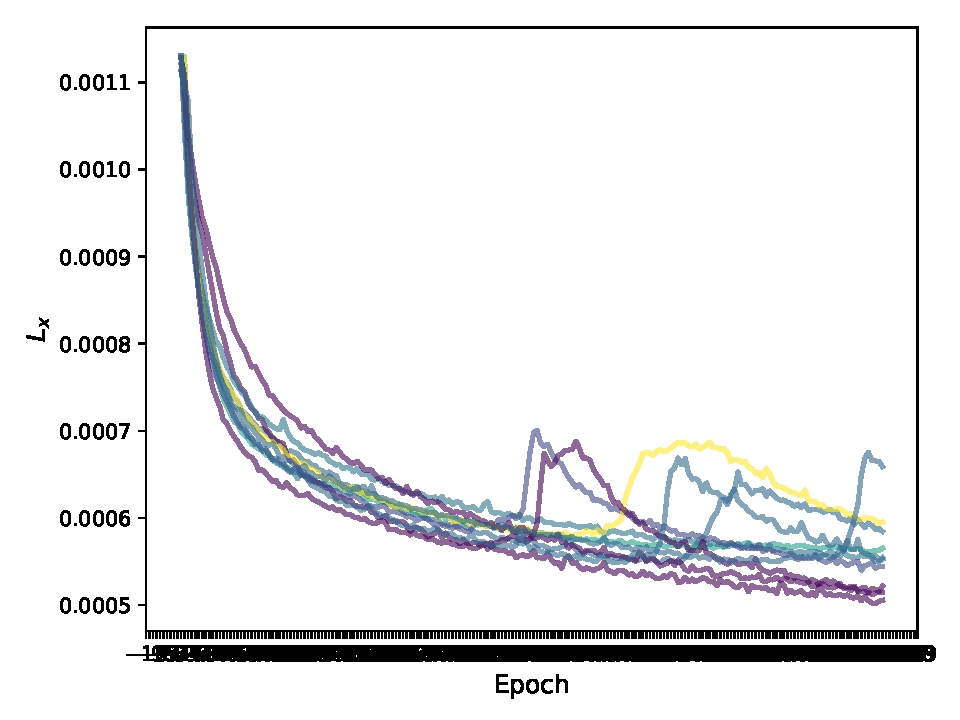
\includegraphics[width=0.9\textwidth]{/plots/reconst_loss.pdf}
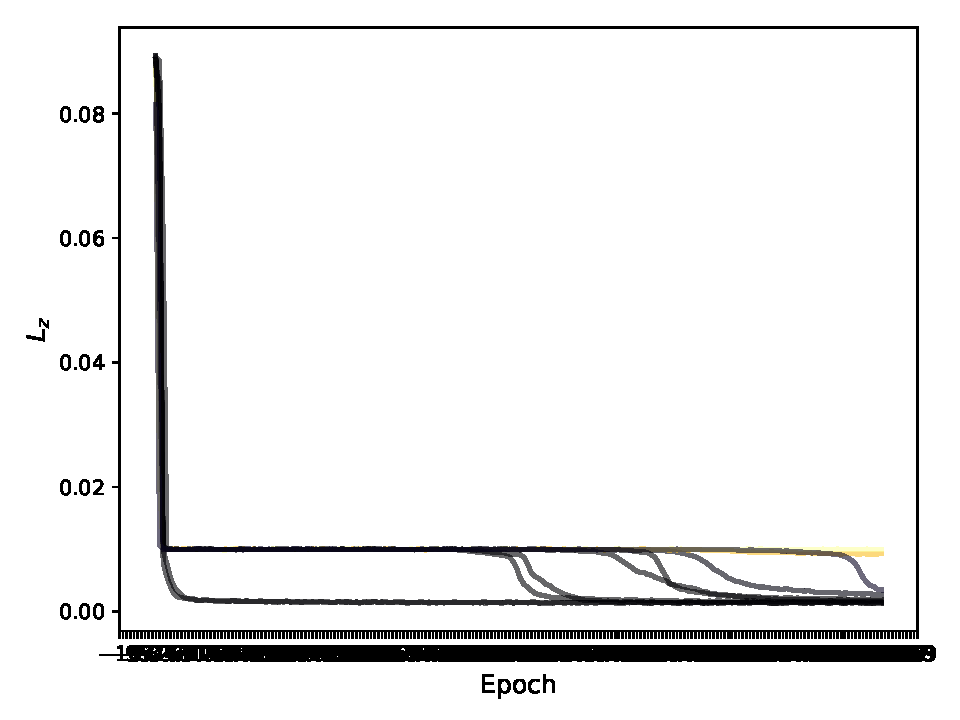
\includegraphics[width=0.9\textwidth]{/plots/latent_loss.pdf}
\caption{Distribution of loss curves for $N=10$ experiments with a convolutional autoencoder. Darkness of color indicates closeness of sample minimum to the population minimum}\label{fig:sim_clf_loss}
\end{figure}